This chapter provides a formal analysis of the system using the Alloy language and a couple of example worlds.

\section{Model}
Below is a code snippet of the model, including signatures, facts and assertions.

\lstinputlisting[language=Alloy]{code/model.als}

\subsection{Example Worlds}
Below are several examples of the model, demonstrating its coherence and correctness with respect to its key functionalities.

\subsection{Base World}
The following base world sets the stage by outlining the domain: two students apply for the same position, one through a recommendation and the other through a direct application. However, only one progresses to the selection process.

\begin{figure}[h]
    \centering
    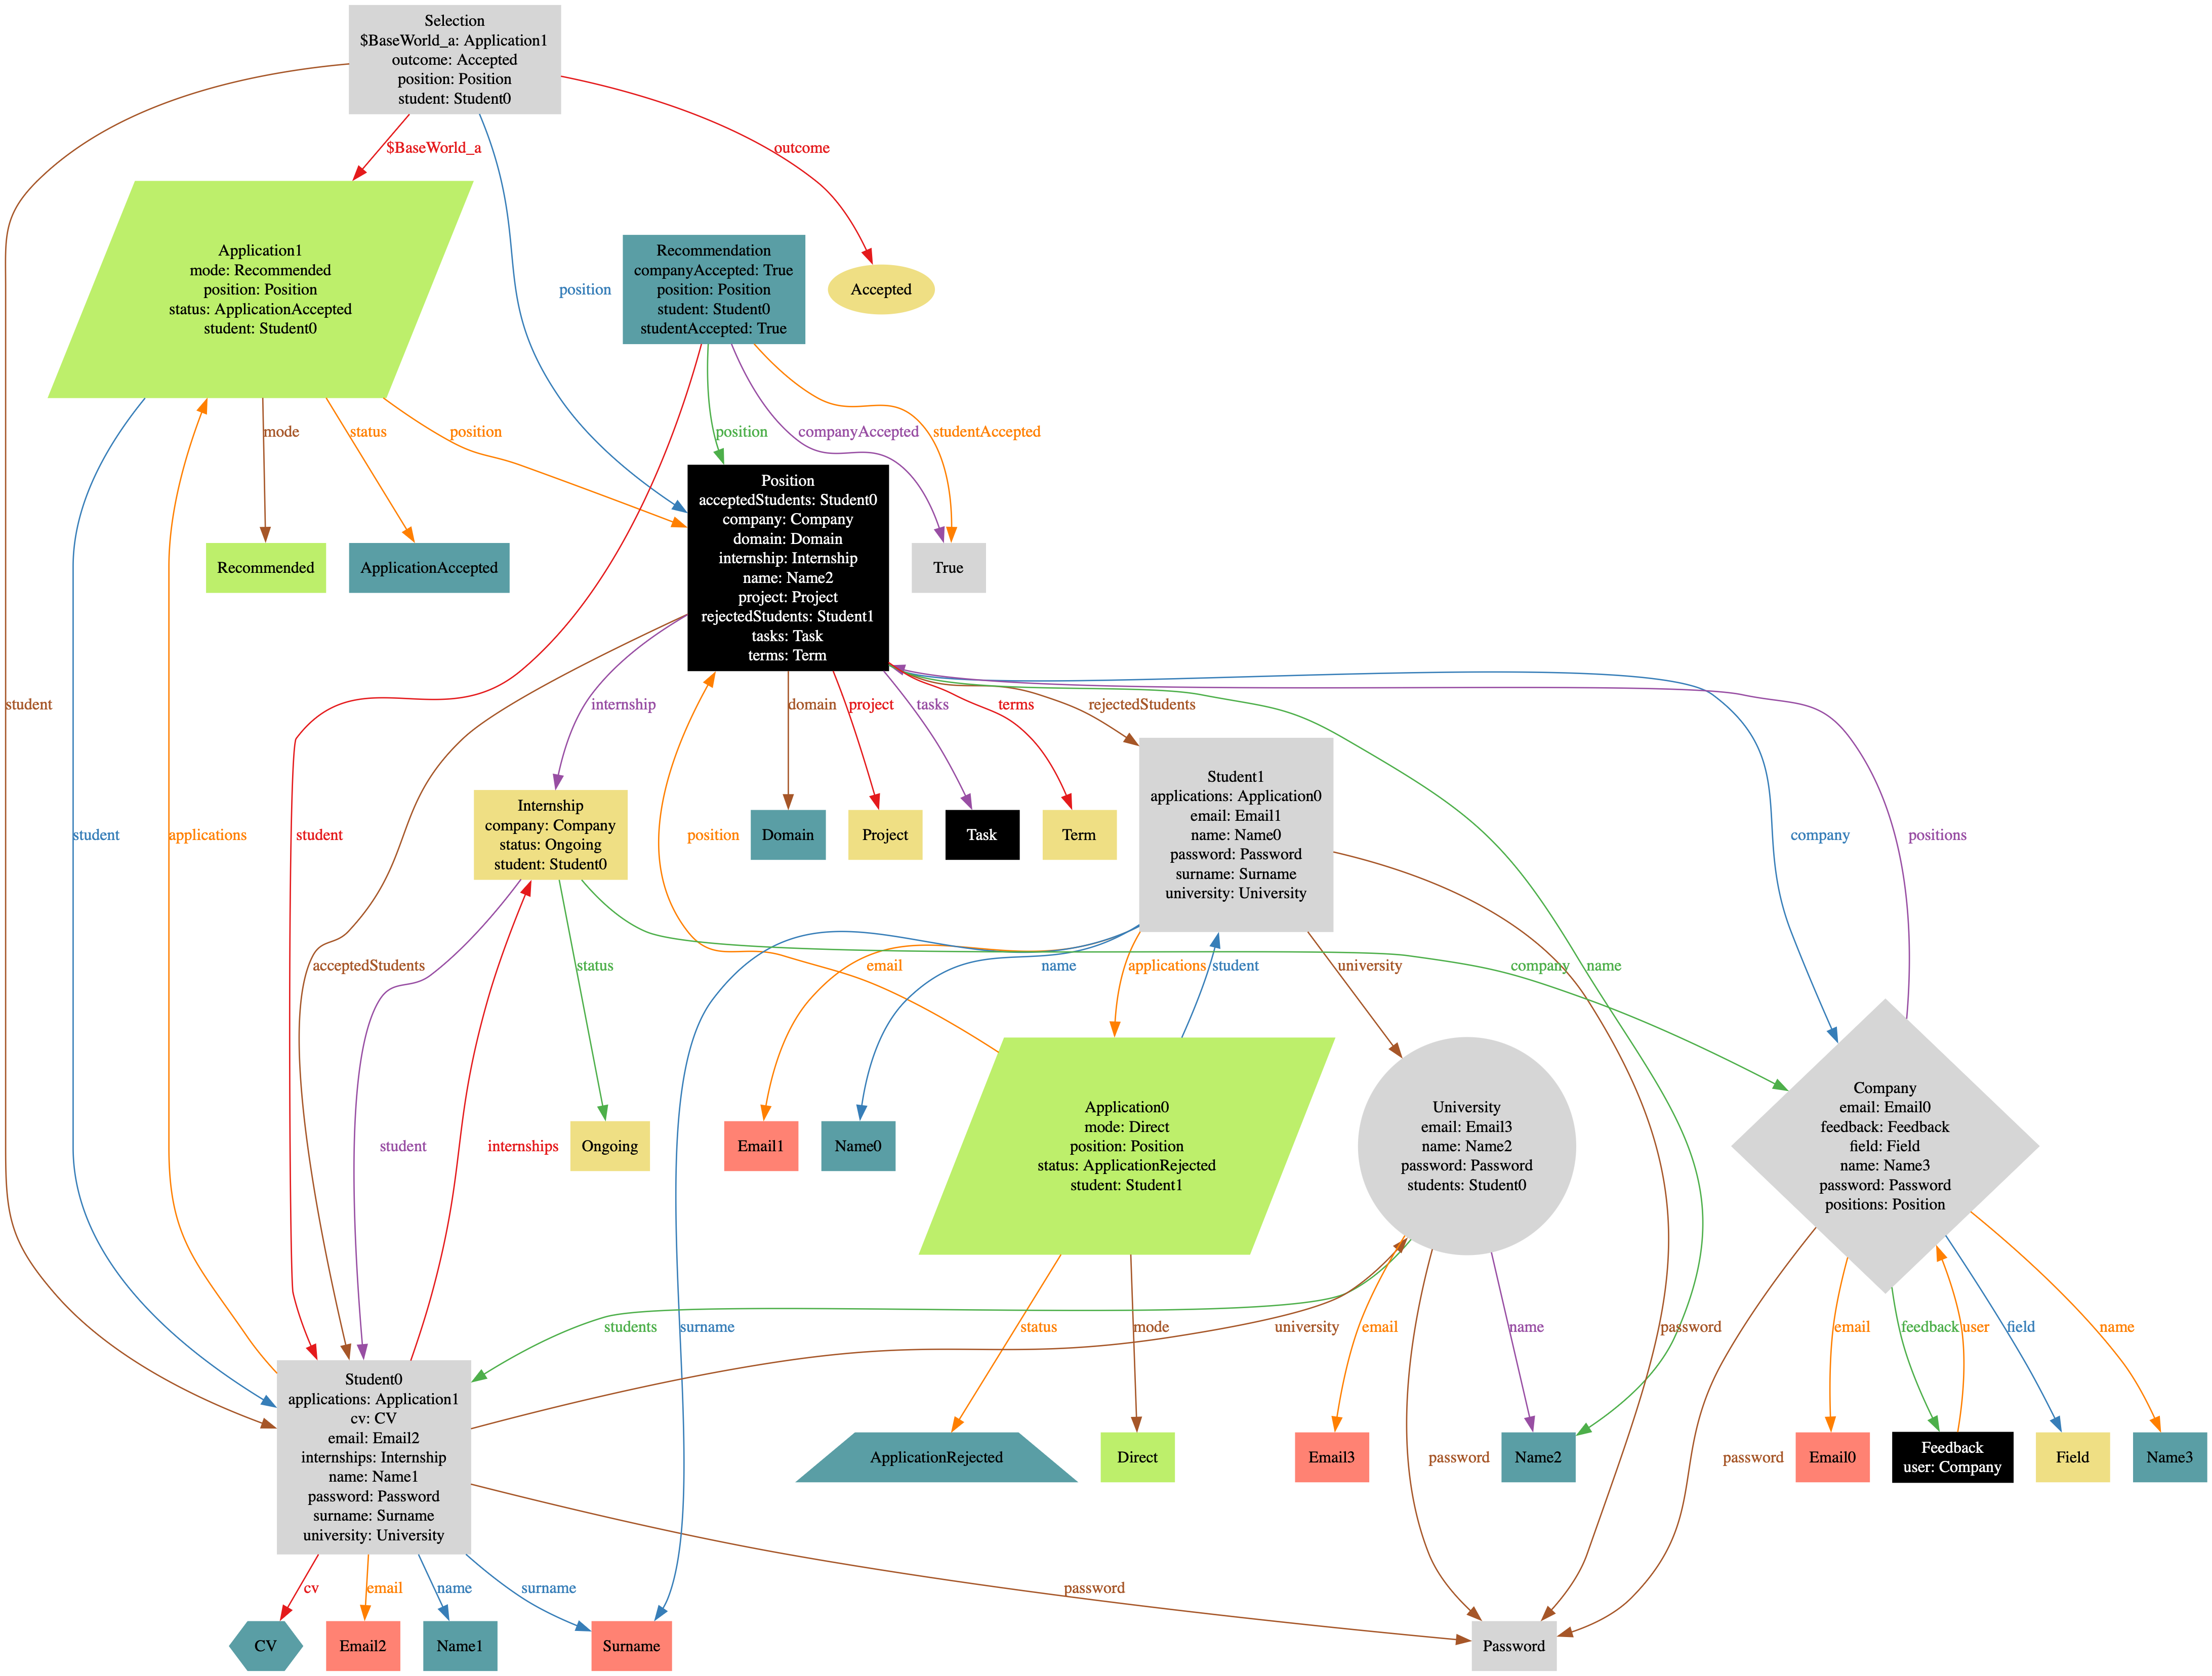
\includegraphics[width=16cm]{images/worlds/base.png}
    \caption{Base world}
\end{figure}

\subsubsection{Second World}
In this world, two students apply for the same position. Both successfully advance to the selection process, but only one ultimately secures the internship.

\begin{figure}[h]
    \centering
    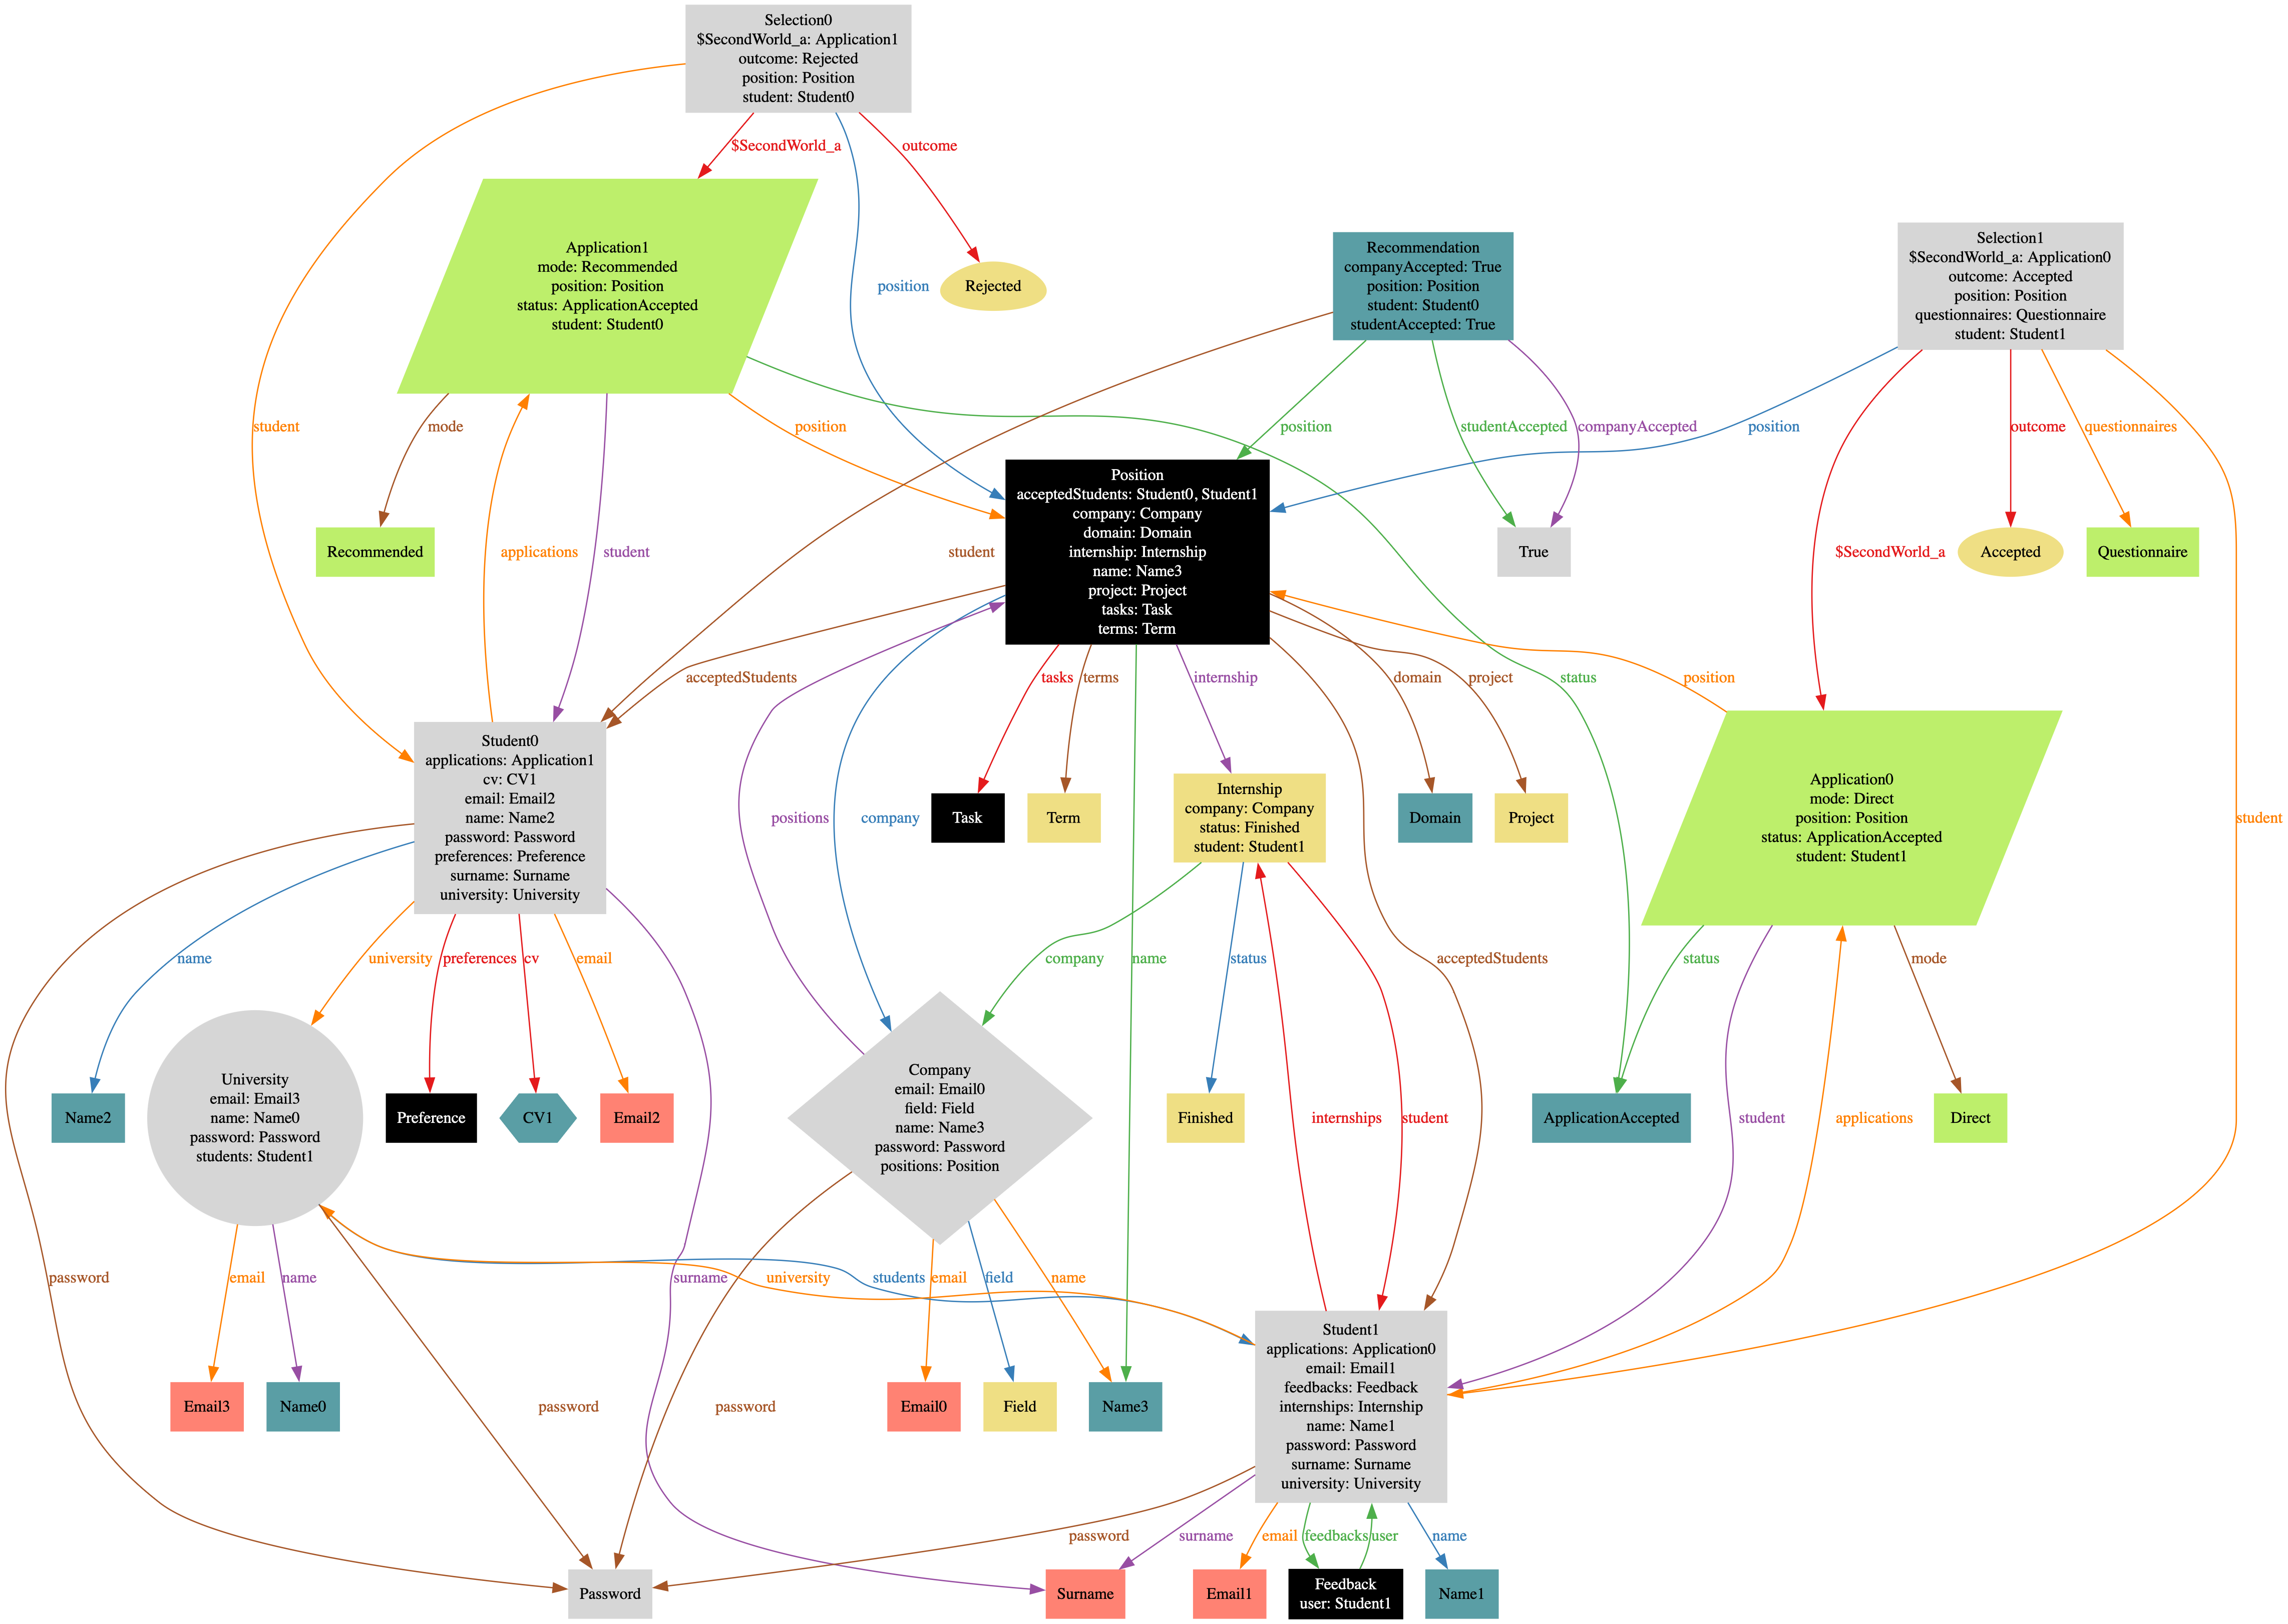
\includegraphics[width=16cm]{images/worlds/second.png}
    \caption{Second world}
\end{figure}
